% Homework Requirements
% - What are the motivations for this work?
% - What is the proposed solution?
% - What is the work’s evaluation of the proposed solution?
% - What is your analysis of the identified problem, idea, and evaluation?
% - What are future directions for this research?
% - What questions are you left with?

\documentclass[12pt]{article}

% Font family
\usepackage{xeCJK}
\setCJKmainfont{Noto Serif TC}
\usepackage{amssymb}
\usepackage{amsmath}

% Document layout
\usepackage[margin=2cm, a4paper]{geometry}
\usepackage{setspace}
\onehalfspacing
\setlength{\parskip}{12pt}
\setlength{\parindent}{0pt}

% Citation
\usepackage{biblatex}
\addbibresource{./ref.bib}

% Image
\usepackage{graphicx}
\graphicspath{{./images/}}

% \title{Paper Review Assignment 1}
% \author{施宇庭}

\begin{document}
% \maketitle

%%%%%%%%%%%%%%%%%%%%%%%%%%%%%%%%%%%%%%%%%%%%%%%%%%%%%%%%%%%%

\begin{titlepage}
\begin{center}

\vspace*{1cm}
\large AOC 2024 Spring \\
\Large Paper Review Assignment 1 \\

\vspace{2cm}
% \LARGE \textbf{Xception: Deep Learning with Depthwise Separable Convolutions} \\
\LARGE \textbf{Review of "An Image is Worth 16X16 Words: Transformers for Image Recognition at Scale"} \\

\vfill
\normalsize
學生:施宇庭 NN6124030 \\ [0.2cm]
指導教授:蔡家齊 \ 助理教授 \\ [0.2cm]

\end{center}
\end{titlepage}

% \pagebreak \tableofcontents \pagebreak

%%%%%%%%%%%%%%%%%%%%%%%%%%%%%%%%%%%%%%%%%%%%%%%%%%%%%%%%%%%%

\section{Motivation}

Transformers have achieved tremendous success in the natural language processing (NLP) field in recent years, thanks to their model design that gives them high scalability. As the dataset scale grows, the model has not yet reached its performance bottleneck.

In the computer vision (CV) field, some research has been trying to combine CNNs with self-attention, while others has completely replaced the convolution layers with self-attention. However, due to the specially designed attention layers not scaling effectively enough, ResNet-like architectures still remained the state-of-the-art (SOTA) for image recognition prior to this paper.

Therefore, this paper aims to address this issue by splitting the image into small patches and input them into the transformer, just like how NLP takes a sequence of words as input. This approach tries to stay as close as possible to the original transformer design, in order to exploit its efficiency and scalability on modern hardware.

%%%%%%%%%%%%%%%%%%%%%%%%%%%%%%%%%%%%%%%%%%%%%%%%%%%%%%%%%%%%

\section{Proposed Method}

\subsection{Model Architecture}

The model architecture of Vision transformer (ViT) is shown in Figure \ref{fig:model_arch}.

To get the input of the transformer encoder:

\begin{enumerate}
    \item Reshape the input image $\mathbf{x} \in \mathbb{R}^{1 \times H \times W \times C}$ to a sequence of 2D patches $\mathbf{x}_p \in \mathbb{R}^{N \times P \times P \times C}$, where $N = HW/P^2$ is the number of patches, and $P$ is the patch size.
    \item Flatten and project each patch $\mathbf{x}_p^i$ to $\mathbf{x}_p^i\mathbf{E} \in \mathbb{R}^D$, where $\mathbf{E} \in \mathbb{R}^{(P^2 \cdot C) \times D}$
    \item Prepend a learnable class token as $\mathbf{x}_p^0$ to the sequence, and plus the positional embedding $\mathbf{E}_\text{pos} \in \mathbb{R}^{(N+1) \times D}$.
\end{enumerate}

This forms the patch embeddings (Eq. \ref{eq:1}).

\begin{equation}
    \mathbf{z_0} = [\mathbf{x}_\text{class}; \mathbf{x}_p^1\mathbf{E}; ...; \mathbf{x}_p^N\mathbf{E}] + \mathbf{E}_\text{pos} \label{eq:1}
\end{equation}

The transformer encoder consists of alternating layers of multihead self-attention (MSA) and multi-layer perceptron (MLP) blocks as shown in \cite{vaswani_attention_2023}. The difference is that the encoder of this paper applies layer normalization (LN) before every block, and residual connections after every block like the Pre-LN archtecture in \cite{xiong_layer_2020}.

\begin{align}
    \mathbf{z'}_{l} &= \text{MSA}(\text{LN}(\mathbf{z}_{l-1})) + \mathbf{z}_{l-1}, & l = 1 ... L \\
    \mathbf{z}_{l} &= \text{MLP}(\text{LN}(\mathbf{z'}_{l})) + \mathbf{z'}_{l}, & l = 1 ... L \\
    \mathbf{y} &= \text{LN}(\mathbf{z}_{l}^0)
\end{align}

Note that the MLP contains two layers with GELU activation function.

\begin{figure}
    \centering
    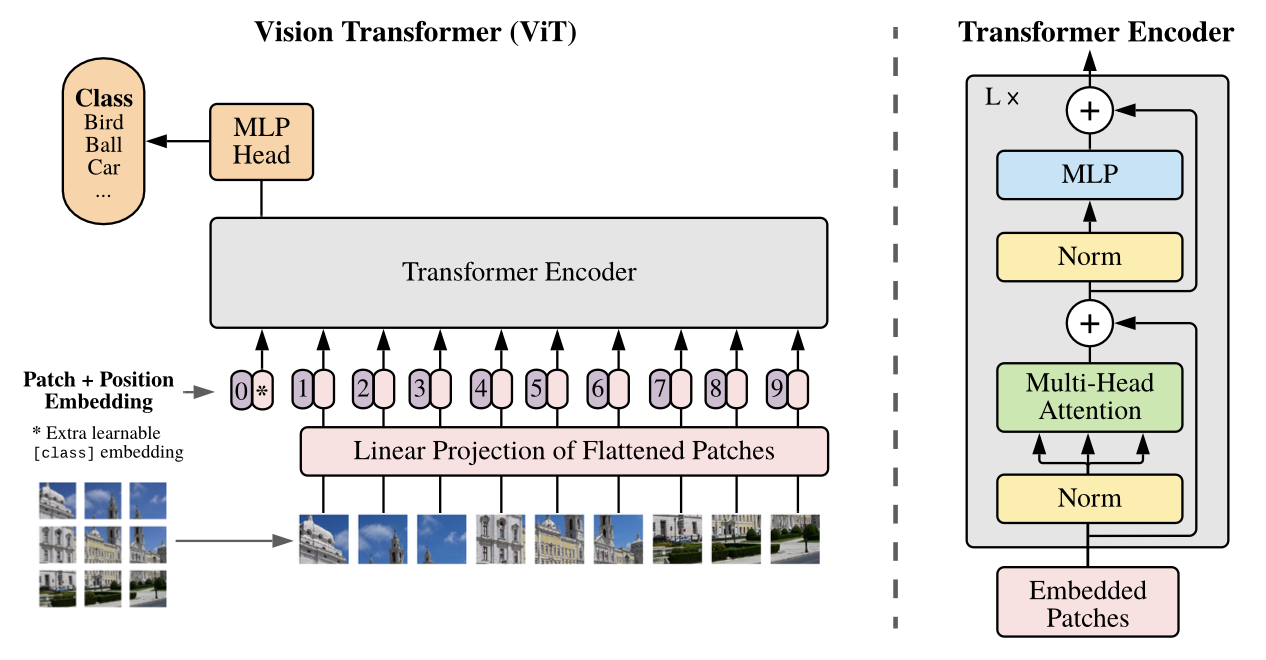
\includegraphics[width=1.0\linewidth]{images/model_arch.png}
    \caption{Model architecture of Vision Transformer \cite{dosovitskiy_image_2021}}
    \label{fig:model_arch}
\end{figure}

%%%%%%%%%%%%%%%%%%%%%%%%%%%%%%%%%%%%%%%%%%%%%%%%%%%%%%%%%%%%

\subsection{Pre-training and Fine-tuning}

This article pre-trains ViT on large datasets, and then fine-tunes to a relatively smaller downstream tasks.

%%%%%%%%%%%%%%%%%%%%%%%%%%%%%%%%%%%%%%%%%%%%%%%%%%%%%%%%%%%%

\section{Experiment and Evaluation}

To demonstrate the effectiveness of the proposed method, this work evaluate the ViT with ResNet-like CNN, and the hybrid.

This paper conducts several experiments to investigate the effectiveness and operation of ViT by:

\begin{enumerate}
    \item Comparing the performance and computational cost of ViT and SOTA CNNs on popular image classification datasets. (Figure \ref{fig:acc_cmp} and \ref{fig:acc_cmp2})
    \item Examining the impact of different pre-training dataset sizes. (Figure \ref{fig:data_size1} and \ref{fig:data_size2})
    \item Assessing the scalability of ViT across different sizes. (Figure \ref{fig:model_vary})
    \item Analyzing the internal operation of ViT.
\end{enumerate}

%%%%%%%%%%%%%%%%%%%%%%%%%%%%%%%%%%%%%%%%%%%%%%%%%%%%%%%%%%%%

% \subsection{Experimental Setup}

%%%%%%%%%%%%%%%%%%%%%%%%%%%%%%%%%%%%%%%%%%%%%%%%%%%%%%%%%%%%

\subsection{Comparison to State of The Art}

To demonstrate the effectiveness of the proposed method, this study compares the accuracy and computational cost (TPUv3-cores-days) of ViT with that of SOTA CNNs on popular image classification datasets. Figure \ref{fig:acc_cmp} shows the results, and we can find that:

\begin{itemize}
    \item A smaller ViT-L/16 pre-trained on JFT-300M outperforms BiT pre-trained on JFT-300M across all tasks.
    \item A larger ViT-H/14 exhibits even better performance than ViT-L/16.
    \item ViTs require fewer computational resources for pre-training compared to other SOTA CNNs.
\end{itemize}

However, pre-training efficiency is influenced not only by the model architecture but also by other factors such as training schedule, optimizer, and weight decay.

\begin{figure}
    \centering
    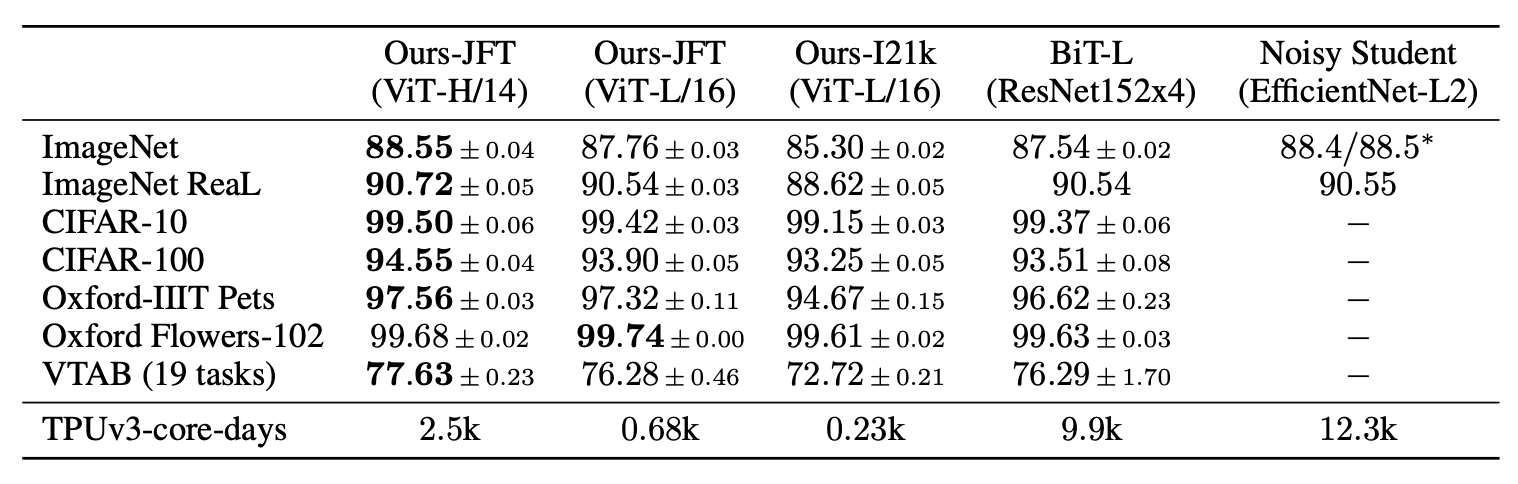
\includegraphics[width=1\linewidth]{images/acc_cmp1.png}
    \caption{Comparison with SOTA CNNs on popular image classification benchmarks.}
    \label{fig:acc_cmp}
\end{figure}

Figure \ref{fig:acc_cmp2} decomposes the VTAB tasks into their respective groups, and compares to previous SOTA methods on this benchmark. ViT-H/14 outperforms BiT-R152x4, and other methods, on the \textit{Natural} and \textit{Structured} tasks. On the Specialized the performance of the top two models is similar.

\begin{figure}
    \centering
    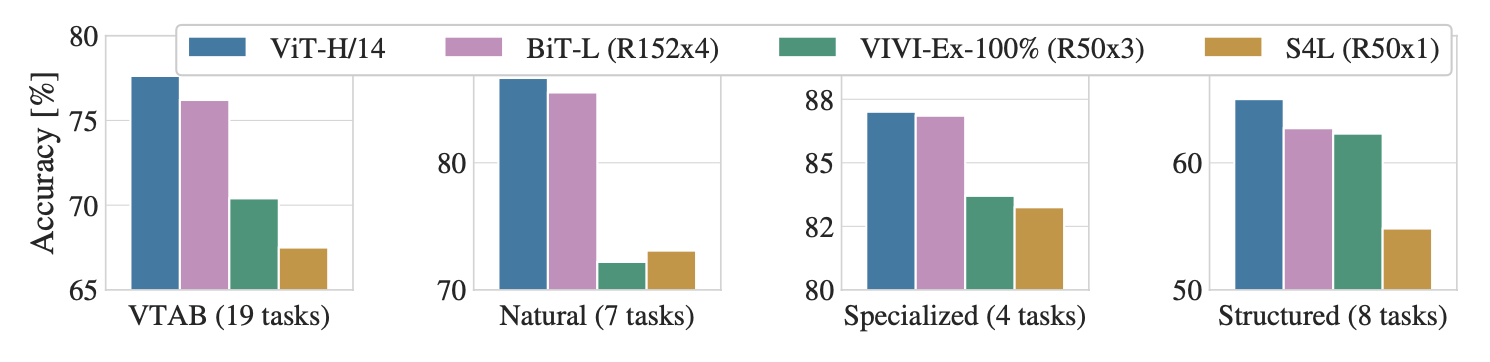
\includegraphics[width=1\linewidth]{images/acc_cmp2.png}
    \caption{Breakdown of VTAB performance in \textit{Natural}, \textit{Specialized}, and \textit{Structured} task groups.}
    \label{fig:acc_cmp2}
\end{figure}

%%%%%%%%%%%%%%%%%%%%%%%%%%%%%%%%%%%%%%%%%%%%%%%%%%%%%%%%%%%%

\subsection{Pre-training Data Requirements}

To investigate how crucial is the dataset size of pre-training, this paper further compared the accuracy of ViT and BiT with varying pre-training dataset sizes: ImageNet, ImageNet-21k, and JFT300M. Figure \ref{fig:data_size1} shows the result after fine-tuning to ImageNet, and the results are:

\begin{itemize}
    \item When pre-trained on small dataset (ImageNet), ViT-Base models are better than ViT-Large models, despite the regularization including weight decay, dropout, and smoothing. And the BiT model outperforms the ViT models.
    \item When pre-trained on medium-sized dataset (ImageNet-21k), their performances are similar.
    \item When pre-trained on large dataset (JFT-300M), larger ViT start revealing the benefit.
\end{itemize}

An additional experiment was performed on random subsets of 9M, 30M, and 90M as well as the full JFT300M dataset. As shown in figure \ref{fig:data_size2}, similar result holds: ResNets perform better with smaller pre-training datasets, while ViT performs better with larger pre-training datasets.

\begin{figure}
    \centering
    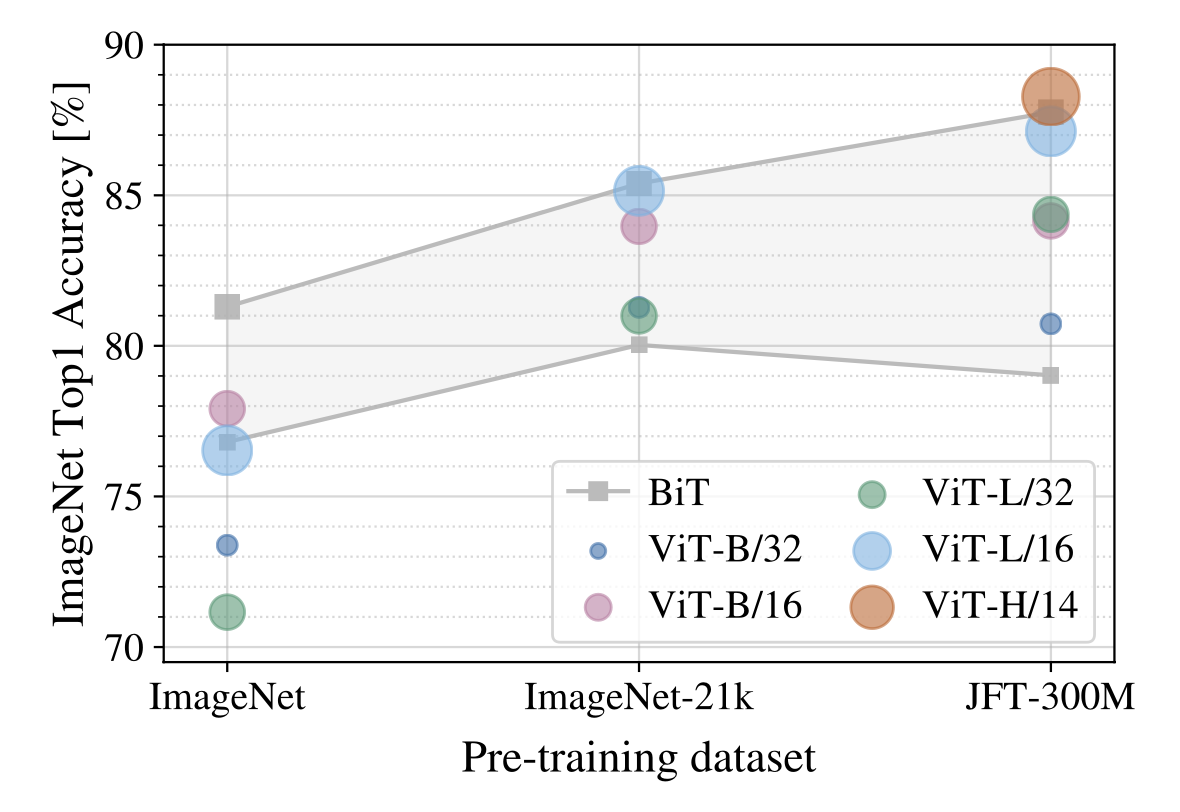
\includegraphics[width=0.7\linewidth]{images/data_size1.png}
    \caption{Transfer to ImageNet.}
    \label{fig:data_size1}
\end{figure}

\begin{figure}
    \centering
    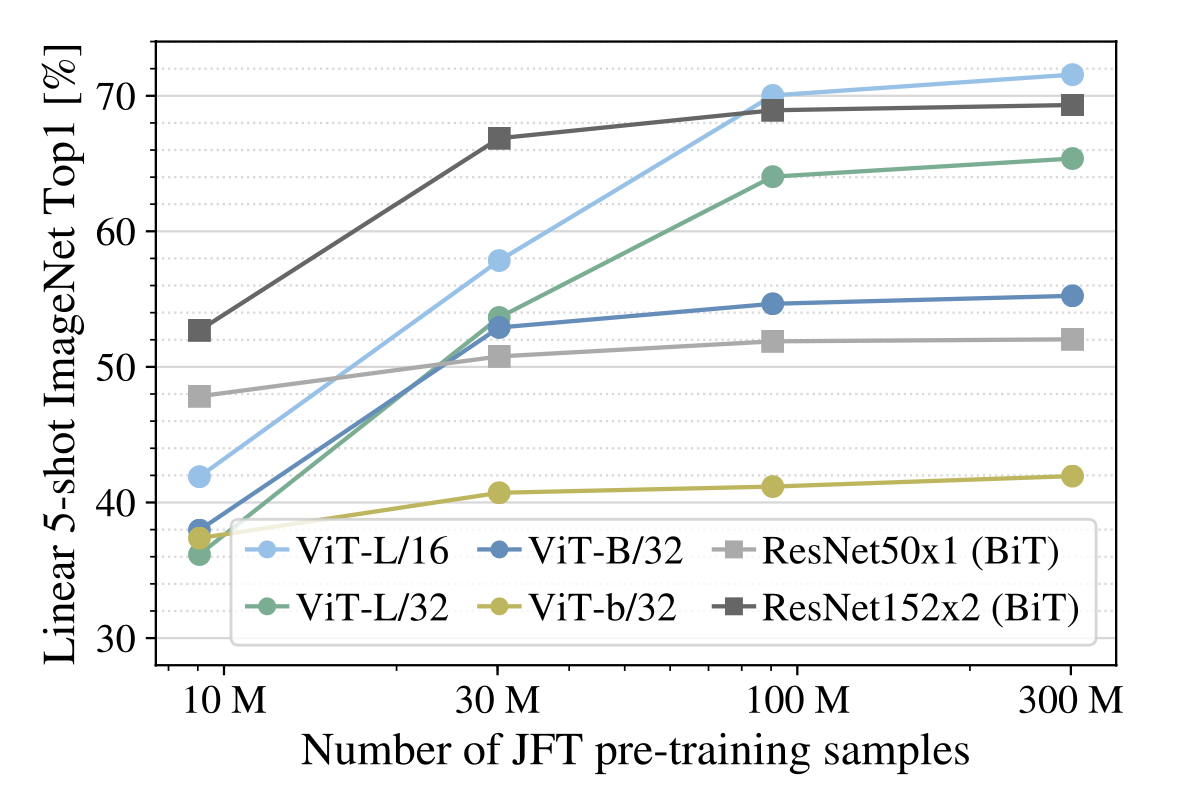
\includegraphics[width=0.7\linewidth]{images/data_size2.png}
    \caption{Linear few-shot evaluation on Ima- geNet versus pre-training size.}
    \label{fig:data_size2}
\end{figure}

%%%%%%%%%%%%%%%%%%%%%%%%%%%%%%%%%%%%%%%%%%%%%%%%%%%%%%%%%%%%

\subsection{Scaling Study}

Observing the transformer performance on JFT-300M with different models allows for an assessment of scalability (performance/compute trade-off). The result is shown in figure \ref{fig:model_vary}.  We can observe that:

\begin{itemize}
    \item ViT dominate ResNets on the performance/compute trade-off.
    \item hybrids slightly outperform ViT at small computational budgets, but the difference vanishes for larger models.
    \item Vision Transformers appear not to saturate within the range tried, motivating future scaling efforts.
\end{itemize}

\begin{figure}
    \centering
    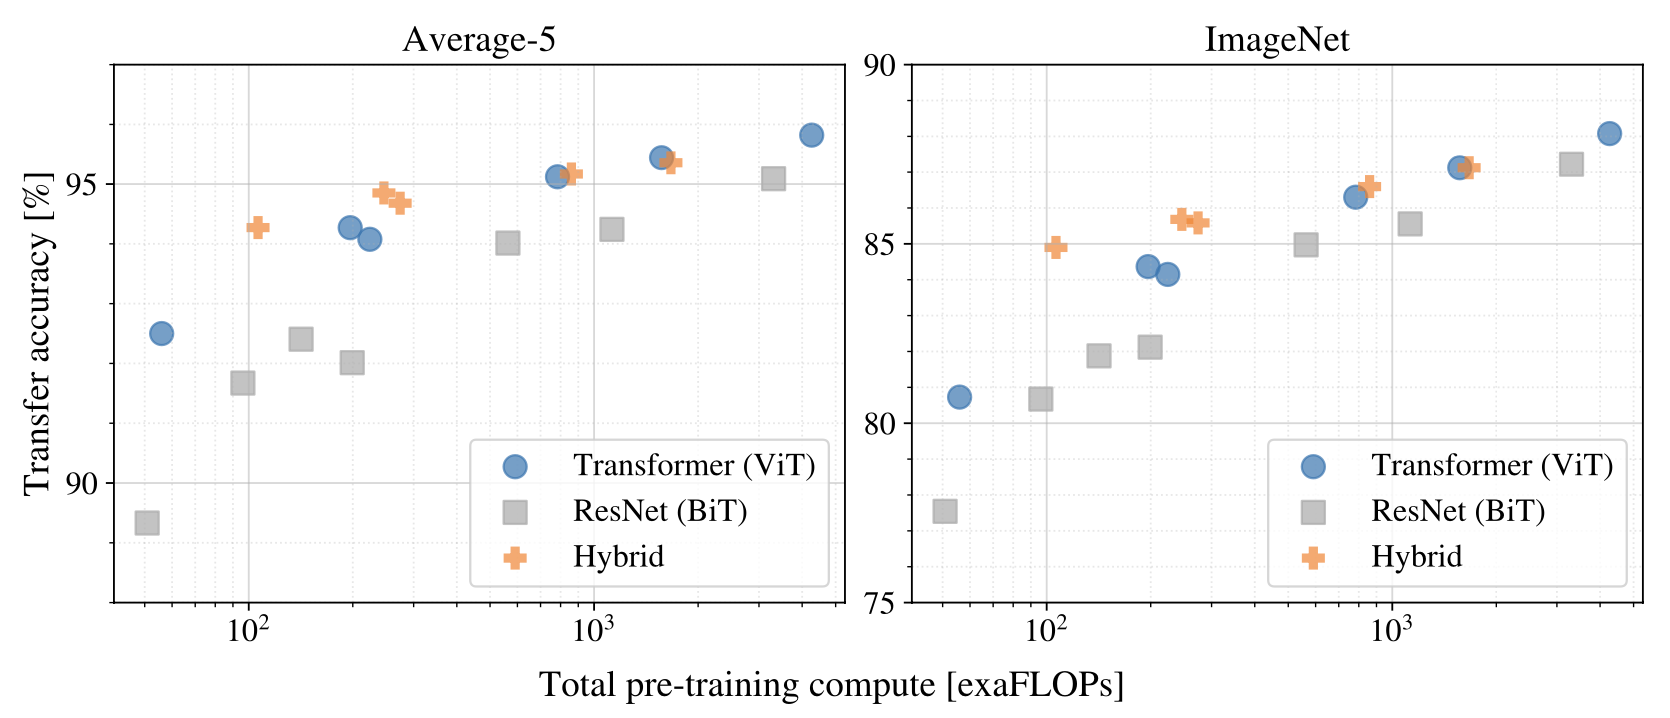
\includegraphics[width=1\linewidth]{images/model_vary.png}
    \caption{Performance versus pre-training compute for different architectures: Vision Transformers, ResNets, and hybrids.}
    \label{fig:model_vary}
\end{figure}

%%%%%%%%%%%%%%%%%%%%%%%%%%%%%%%%%%%%%%%%%%%%%%%%%%%%%%%%%%%%

% \subsection{Inspecting Vision Transformer}

%%%%%%%%%%%%%%%%%%%%%%%%%%%%%%%%%%%%%%%%%%%%%%%%%%%%%%%%%%%%

% \subsection{Self-Supervision}

%%%%%%%%%%%%%%%%%%%%%%%%%%%%%%%%%%%%%%%%%%%%%%%%%%%%%%%%%%%%

\section{Analysis}

\subsection{Pre-LN v.s. Post-LN Transformer}

When reviewing the relevant literature, I noticed that the encoder architecture proposed in this paper differs slightly from the original transformer architecture. The original model architecture of transformer proposed by \cite{vaswani_attention_2023} is shown in figure \ref{fig:model_arch_orig}. Comparing with the figure \ref{fig:model_arch}, we can observe that the relative position of the layer normalization differs. In the original paper, the LN layer comes after the MSA and MLP, while in this paper, the LN layer comes before the MSA and MLP. In this paper, the rationale behind such a design choice is not explicitly discussed. However, a study by \cite{xiong_layer_2020} suggests that in the original paper, the Post-LN approach results in larger gradients near the output layer, leading to instability during training with larger learning rates. Consequently, an additional warm-up stage is required, introducing more variability in experiments (unlike the training procedure of CNNs). In contrast, employing Pre-LN results in smaller gradients, making it more suitable for deep neural networks and eliminating the need for a warm-up stage.

\begin{figure}
    \centering
    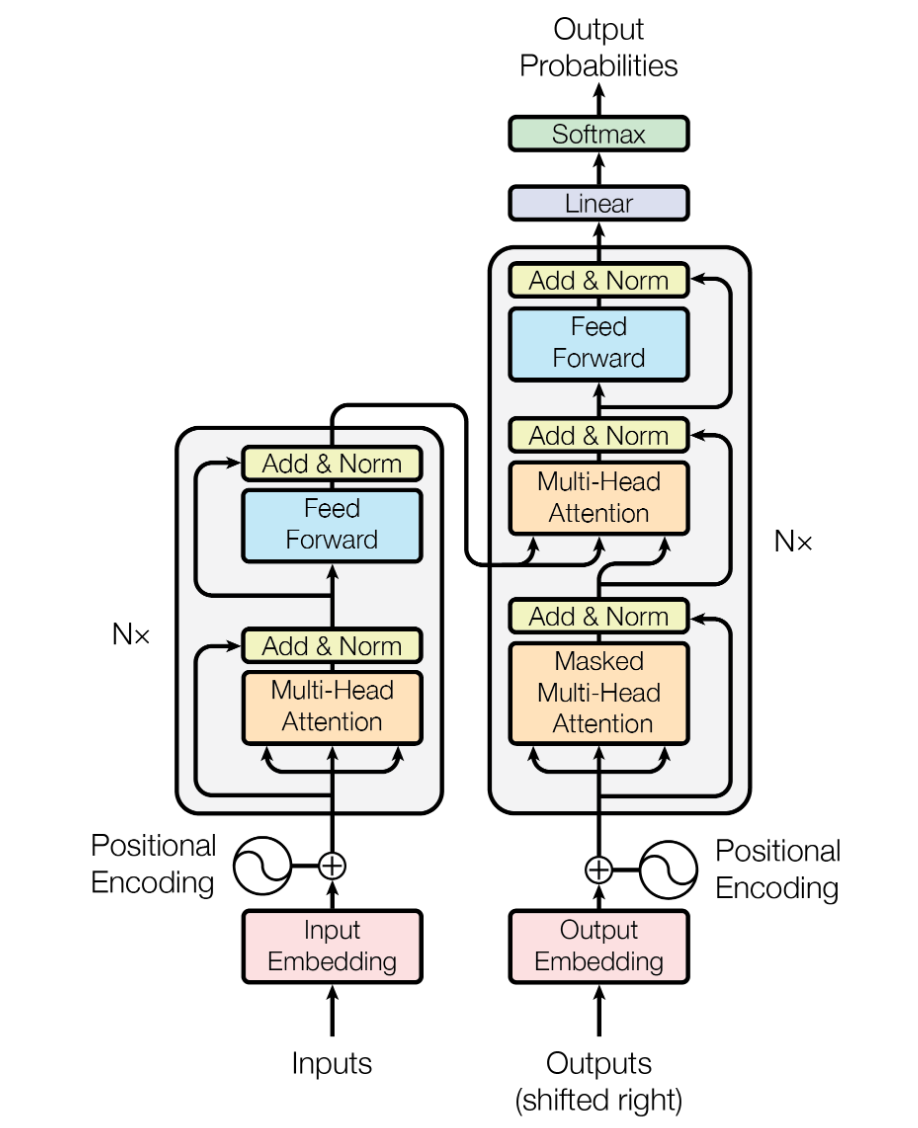
\includegraphics[width=0.5\linewidth]{images/model_arch_orig.png}
    \caption{The original model architecture of transformer proposed by \cite{vaswani_attention_2023}}
    \label{fig:model_arch_orig}
\end{figure}

%%%%%%%%%%%%%%%%%%%%%%%%%%%%%%%%%%%%%%%%%%%%%%%%%%%%%%%%%%%%

% \subsection{}

%%%%%%%%%%%%%%%%%%%%%%%%%%%%%%%%%%%%%%%%%%%%%%%%%%%%%%%%%%%%

\section{Future Work}

The authors proposed some future work for this research including:

\begin{enumerate}
    \item Applying to other computer vision tasks (e.g. detection, segmentation)
    \item Large-scale self-supervised pre-training
    \item Further scaling on ViT
\end{enumerate}


In addition to the directions proposed by the authors, I believe there are the following directions for future development:

Transformer models have a vast number of parameters and computations, typically trained and inferred on servers. However, even on servers, there is a demand for model compression to save computation costs and increase throughput \cite{zhao_atom_2023}. ViT models used in the field of computer vision are no exception. However, traditional quantization and pruning techniques for CNNs may not be directly applicable to transformer model computations. Therefore, developing quantization algorithms suitable for ViT would be a promising research direction. For example, there is already research on post-training quantization (PTQ) for ViT \cite{liu_post-training_2021}. However, quantization-aware training (QAT) for ViT remains an unresolved issue due to training oscillations causing instability during the training process.

This paper proposes a redesign of the algorithm to enable transformers to efficiently perform computer vision tasks using existing hardware (TPUv3). It also points out that previous papers have not performed well due to the under-utilization of hardware capabilities caused by specific attention patterns. Furthermore, experimental results indicate that existing large datasets have not reached the limit of Vision Transformer and still have the potential for further scaling up. Therefore, developing a software/hardware co-design system for ViT is also a research direction worth exploring.

%%%%%%%%%%%%%%%%%%%%%%%%%%%%%%%%%%%%%%%%%%%%%%%%%%%%%%%%%%%%

% \pagebreak
\printbibliography
\end{document}
